\documentclass[tikz,border=10pt]{standalone}
\usetikzlibrary{calc}

\begin{document}
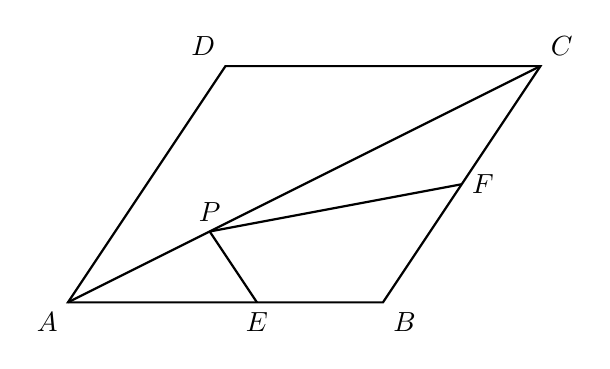
\begin{tikzpicture}[scale=2, thick]
    % 1. 定义顶点坐标 (平行四边形 ABCD)
    \coordinate (A) at (0,0);
    \coordinate (B) at (2,0);
    \coordinate (D) at (1,1.5);
    \coordinate (C) at ($(B)+(D)-(A)$); % 通过向量计算得出C点

    % 2. 定义内部点 P, E, F
    % P 位于 AC 上，大约在 1/3 处
    \coordinate (P) at ($(A)!0.3!(C)$);
    % E 在 AB 上
    \coordinate (E) at ($(A)!0.6!(B)$);
    % F 在 BC 上
    \coordinate (F) at ($(B)!0.5!(C)$);

    % 3. 绘制路径
    \draw (A) -- (B) -- (C) -- (D) -- cycle; % 平行四边形主体
    \draw (A) -- (C); % 对角线
    \draw (P) -- (E); % 连接 PE
    \draw (P) -- (F); % 连接 PF

    % 4. 标注点位
    \node[below left]  at (A) {$A$};
    \node[below right] at (B) {$B$};
    \node[above right] at (C) {$C$};
    \node[above left]  at (D) {$D$};
    \node[above]       at (P) {$P$};
    \node[below]       at (E) {$E$};
    \node[right]       at (F) {$F$};

\end{tikzpicture}
\end{document}